\begin{figure}[!h] 
  \begin{subfigure}[b]{0.5\linewidth}
    \centering
    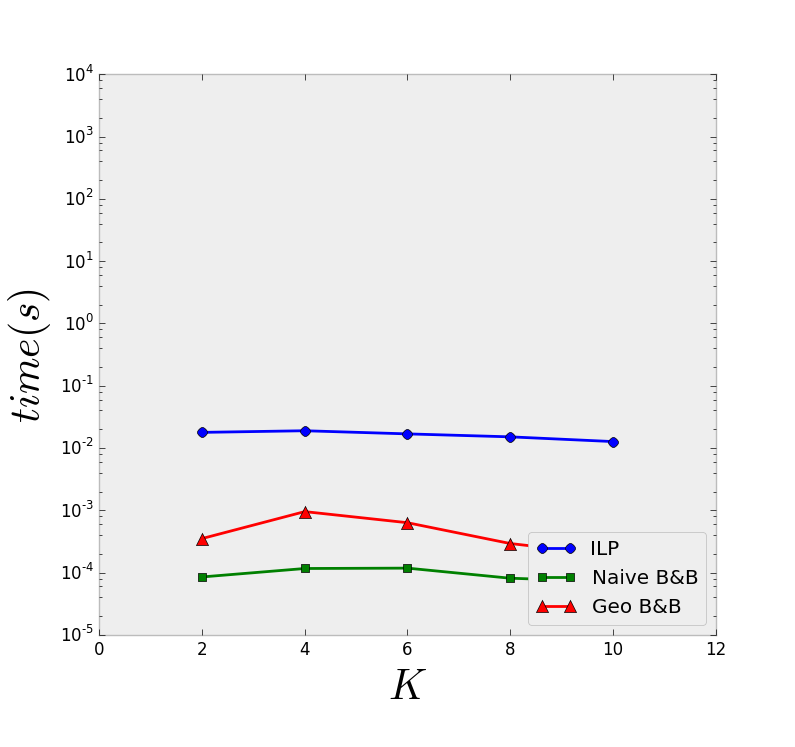
\includegraphics[width=0.9\linewidth]{Pictures/n10} 
    \caption{$N=10$} 
    \label{fig:fixed_n:a} 
  \end{subfigure}%% 
  \begin{subfigure}[b]{0.5\linewidth}
    \centering
    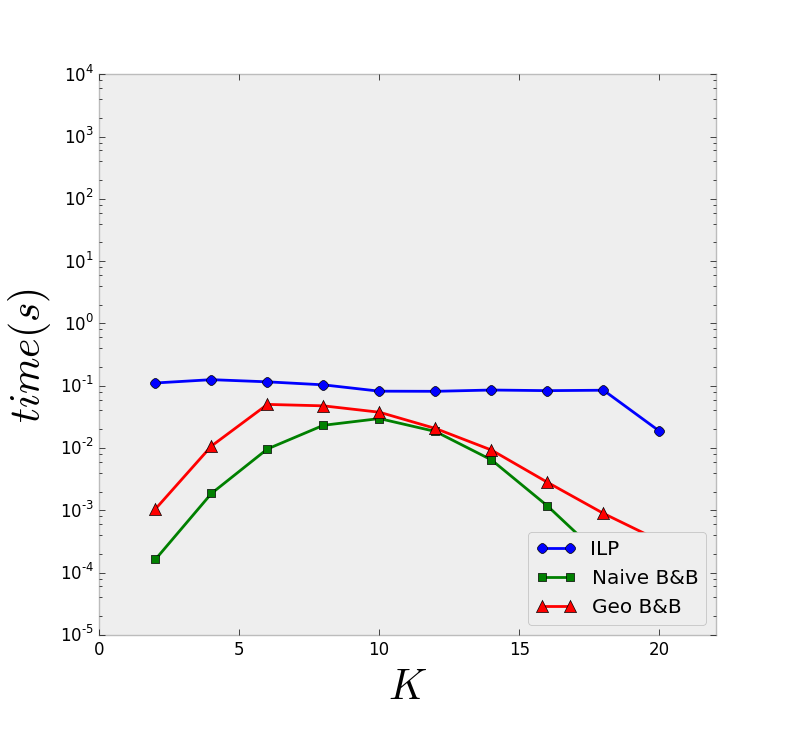
\includegraphics[width=0.9\linewidth]{Pictures/n20} 
    \caption{$N=20$} 
    \label{fig:fixed_n:b} 
  \end{subfigure} 
  \begin{subfigure}[b]{0.5\linewidth}
    \centering
    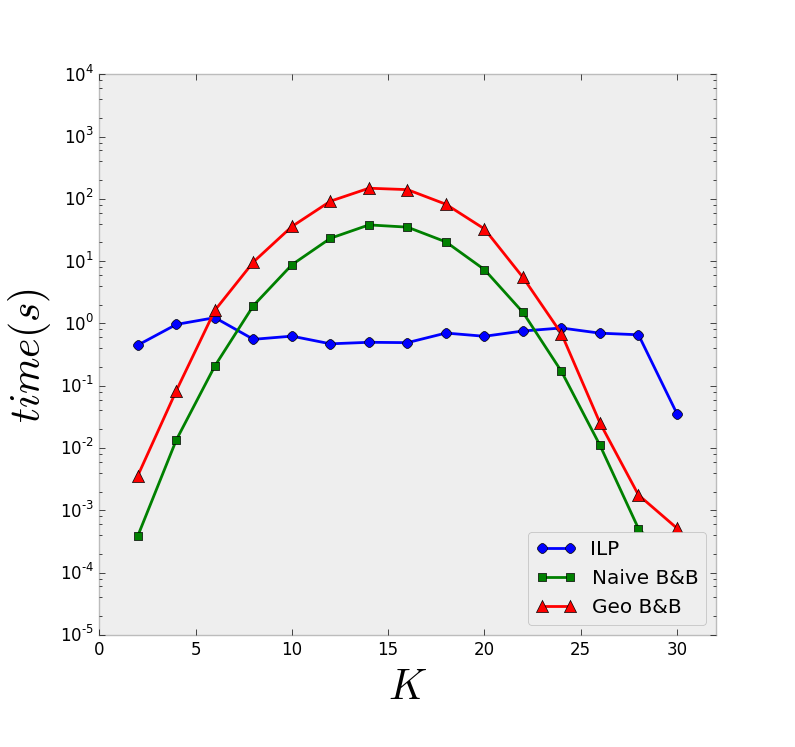
\includegraphics[width=0.9\linewidth]{Pictures/n30} 
    \caption{$N=30$} 
    \label{fig:fixed_n:c} 
  \end{subfigure}%%
  \begin{subfigure}[b]{0.5\linewidth}
    \centering
    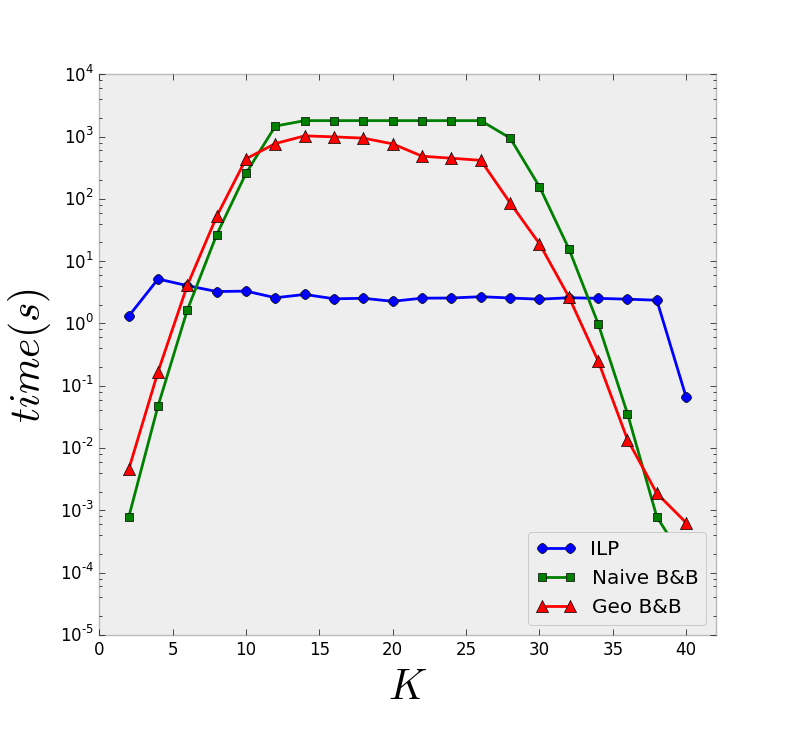
\includegraphics[width=0.9\linewidth]{Pictures/n40} 
    \caption{$N=40$} 
    \label{fig:fixed_n:d} 
  \end{subfigure} 
  \vspace{2ex}
  \begin{center}
  \textcolor{blue}{\cmark}\ -- Integer Linear Programming \quad   \textcolor{red}{\tmark}\ -- Delaunay Assisted B\&B\quad \textcolor{OliveGreen}{\smark}\ -- Naive B\&B
  \end{center}
  \caption{CPU-time for different values of $N$ with varying values of $K$}
  \label{fig:fixed_n} 
\end{figure}

